\documentclass[11pt]{article}

\ifdefined\ARXIVVERSION
\usepackage[preprint]{acl}
\else
\usepackage[review]{acl}
\fi
\usepackage{times}
\usepackage{latexsym}
\usepackage{amsmath}
\usepackage{booktabs}
\usepackage{graphicx}
\usepackage{float}
\usepackage{placeins}
\usepackage[T1]{fontenc}
\usepackage[utf8]{inputenc}
\usepackage{microtype}
\usepackage{inconsolata}
\usepackage{url}
\ifdefined\ARXIVVERSION
\usepackage{orcidlink}
\fi

\newsavebox{\promptboxcontent}
\newenvironment{promptbox}[1]{%
  \par\smallskip
  \begingroup
  \def\promptboxtitle{#1}%
  \setlength{\fboxsep}{0pt}%
  \begin{lrbox}{\promptboxcontent}%
  \begin{minipage}{\dimexpr\linewidth-2\fboxrule\relax}
  \colorbox{black!55}{\makebox[\linewidth][l]{\hspace{6pt}%
    \color{white}\bfseries\small\strut\promptboxtitle}}%
  \par\vspace{6pt}
  \hspace*{6pt}\begin{minipage}{\dimexpr\linewidth-12pt\relax}
  \small\setlength{\parindent}{0pt}
}{%
  \end{minipage}\par\vspace{6pt}
  \end{minipage}%
  \end{lrbox}%
  \noindent\fcolorbox{black!55}{black!2}{\usebox{\promptboxcontent}}%
  \endgroup
  \par\smallskip
}

\title{Query Expansion Should Be Coordinated: Dense Expands, Sparse Anchors}

\ifdefined\ARXIVVERSION
\author{
  Chunran Zhang\,\orcidlink{0009-0005-8865-2090} \\
  School of Computing and Artificial Intelligence \\
  Southwest Jiaotong University \\
  Chengdu, China \\
  \texttt{chronis@my.swjtu.edu.cn}
}
\else
\author{Anonymous ACL submission}
\fi

\providecommand{\tightlist}{\setlength{\itemsep}{0pt}\setlength{\parskip}{0pt}}
\begin{document}
\maketitle

\begin{abstract}
% Generated from markdown/01.abstract.md; edit the Markdown source.
Retrieval-augmented generation (RAG) systems rely on retrieval modules to ground large language model (LLM) outputs. LLM-based query expansion enriches retrieval with document-like passages, but evaluations of hybrid retrieval often fuse fixed top-\(L\) prefixes of dense and sparse rankings. Because \(L\) controls cross-channel contributions and ranking access, it can alter measured expansion gains. We therefore evaluate complete-list effectiveness and record per-channel replay stopping depths required to certify the ordered top-\(K\). This changes the design: because both rankings determine the fused result, their query constructions should be coordinated rather than designed independently. We present DESA (Dense Expansion and Sparse Anchoring), which shares generated references across channels but specializes their integration. Orthogonal residual expansion adds new semantic directions to the dense query, whereas score-product anchoring reorders the original sparse support without admitting expansion-only matches. The same references thus play complementary roles: Dense expands; Sparse anchors. Across seven BEIR datasets, DESA improves nDCG@10 and Recall@20 over the unexpanded query by 3.82\% and 2.38\%, while reducing dense and sparse replay stopping depths by 36.90\% and 36.56\%.

\end{abstract}

% Generated from markdown/02.introduction.md; edit the Markdown source.
\section{Introduction}

\label{sec:introduction}

LLM-based query expansion in hybrid retrieval is commonly evaluated by fusing fixed top-\(L\) prefixes from dense and sparse rankings \citep{gao-etal-2023-precise, wang-etal-2023-query2doc, zhang-etal-2024-exploring-best, liu-zhang-2025-exp4fuse}. Yet \(L\) controls both ranking access and which cross-channel contributions enter fusion, so changing it may change the fused result itself. We instead evaluate effectiveness from the complete rankings, then replay them to record the per-channel depths needed to certify the same ordered top-\(K\). This separates the result produced by an expansion from the ranked evidence required to establish it. We ask whether query expansion can improve the former while reducing both depths relative to the unexpanded query.

\begin{figure}[!t]
  \centering
  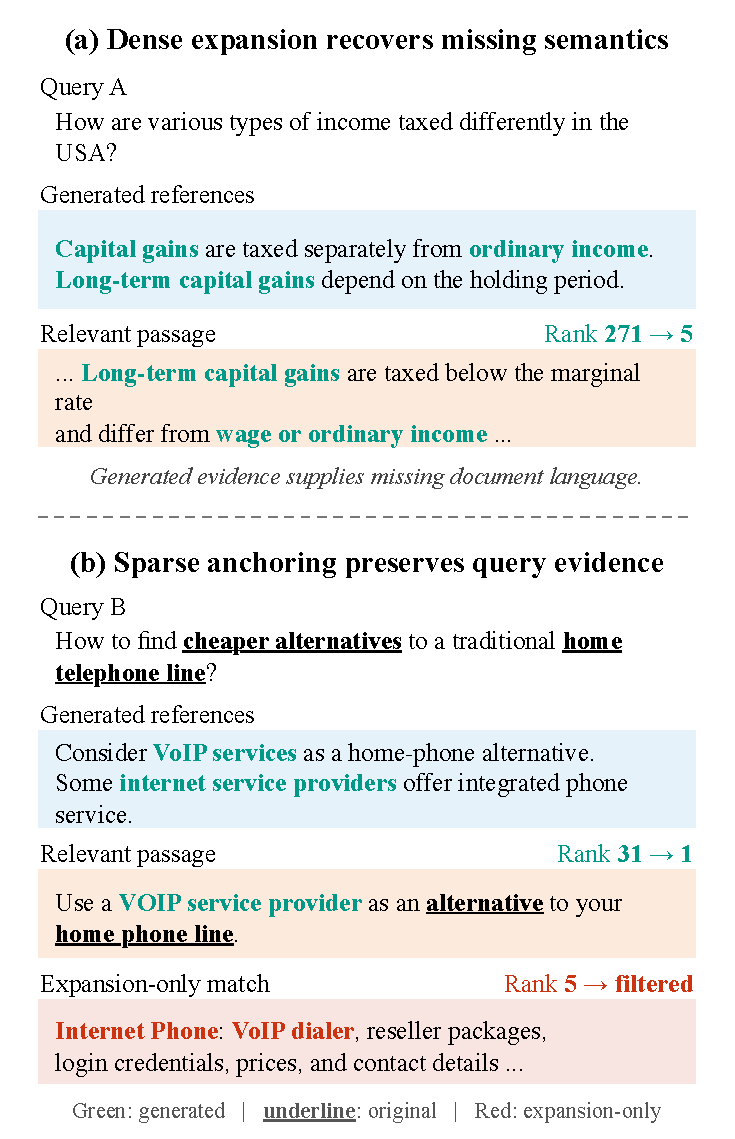
\includegraphics[width=\columnwidth]{figures/fig_desa_intuition.pdf}
  \caption{FiQA examples of DESA \citep{maia-etal-2018-fiqa, thakur-etal-2021-beir}. Dense expansion recovers missing document semantics; sparse anchoring promotes jointly supported passages and excludes expansion-only matches. Two references are shown per query; text is abridged and paraphrased, and ranks use draw~0.}
  \label{fig:desa-intuition}
\end{figure}

This evaluation view changes the design problem. The fused result and the depths required to certify it depend jointly on the dense and sparse rankings, so query construction for the two channels cannot be designed independently. Retriever-specific rewriting adapts each query to its own retriever, but does not explicitly control the cross-channel relation that governs exact fusion \citep{li-etal-2026-dvcqr}. We instead couple the two constructions through one shared set of generated references. Shared generation alone, however, is insufficient: applied directly to both channels, it enlarges sparse support on six of seven datasets, by as much as \(5.72\times\), and on NFCorpus reduces dense depth while increasing sparse depth. These observations motivate a coupled design that shares the evidence basis across channels but constrains its role within each channel.

DESA (Dense Expansion and Sparse Anchoring) implements this shared-generation, channel-specific-integration design. The LLM generates complementary reference passages once and supplies the same references to both channels. In dense retrieval, orthogonal residual expansion preserves the original query direction while adding the new semantic component supplied by the references. In sparse retrieval, score-product anchoring allows the references to reorder originally supported documents without introducing expansion-only matches. Together, these operators coordinate the two channels through shared evidence: dense retrieval can acquire new semantic support, while sparse retrieval remains anchored to the original query support (Figure~\ref{fig:desa-intuition}).

Across seven BEIR datasets, DESA improves equal-dataset macro nDCG@10 and Recall@20 over the unexpanded query by 3.82\% and 2.38\%, while reducing dense and sparse depths by 36.90\% and 36.56\%, respectively. With equal dataset weighting, 63.31\% of queries become shallower in both channels. Compared with matched Shared expansion, DESA significantly improves nDCG while preserving the original sparse support. Component analyses identify sparse anchoring as the more consistent source of effectiveness gains, with dense expansion providing complementary gains across most datasets.

\input{sections/02-related-work}
\section{DESA}
\label{sec:method}

\subsection{Coupled Construction Overview}

DESA jointly designs dense and sparse query construction for the fused result,
aiming to improve complete-list effectiveness while reducing both certification
depths relative to the unexpanded query. Given an original query $q_o$, DESA
first generates one set of complementary reference passages
$R=\{r_1,\ldots,r_n\}$ shared by both channels. This common evidence basis
prevents channel differences from originating in independently generated
rewrites, placing specialization entirely in integration. Dense retrieval may
incorporate new semantic directions from the references, whereas sparse
retrieval may only reorder documents supported by the original query. The
resulting dense and sparse rankings are fused into the final result.
Figure~\ref{fig:desa-overview} summarizes this coupled construction.

\begin{figure}[H]
  \centering
  
\includegraphics[width=\columnwidth]{figures/fig_desa_overview.pdf}
  \caption{Coupled construction in DESA. A shared reference set establishes a
  common evidence basis. Orthogonal residual expansion adds new dense semantic
  directions, whereas score-product anchoring restricts sparse reordering to
  the original query's support.}
  \label{fig:desa-overview}
\end{figure}

\subsection{Shared Reference Generation}

DESA generates one reference set before constructing either channel ranking,
rather than producing a separate rewrite for each retriever. The generated
evidence is therefore held common across channels, so their differences arise
from controlled integration rather than different generated content.

The generator is prompted to produce $n$ short passages that could plausibly
occur in relevant documents. Each passage introduces a different alias,
technical term, or paraphrase while retaining the entities, relations,
numbers, polarity, temporal conditions, scope, and other constraints of
$q_o$. The prompt prohibits broader information needs and invented answers.
The passages therefore vary in expression rather than intent. The same set
$R$ is supplied unchanged to both channel operators. The complete prompt and
decoding settings are provided in Appendix~A.

\subsection{Coupled Dense--Sparse Construction}

The two operators act on the same original query and generated references but
assign different roles to the shared evidence. Dense retrieval permits the
references to add semantic information, subject to bounded deviation from the
original query. Sparse retrieval permits them to alter ranking order, but not
to admit documents unsupported by the original query.

\subsubsection{Orthogonal Residual Expansion}

The dense branch should incorporate semantic information absent from the
original query without allowing the generated references to replace its
original direction. Let $f_D$ be the dense encoder. We encode the original
query and each query--reference pair as unit vectors:

\[
\begin{aligned}
\mathbf v_o&=\operatorname{norm}(f_D(q_o)),\\
\mathbf v_i&=\operatorname{norm}
\!\left(f_D(\operatorname{concat}(q_o,r_i))\right),\\
\bar{\mathbf v}_r&=\frac{1}{n}\sum_{i=1}^{n}\mathbf v_i .
\end{aligned}
\]

We remove the component of $\bar{\mathbf v}_r$ parallel to the original query
and add the remaining residual to $\mathbf v_o$:

\[
\mathbf z=
\bar{\mathbf v}_r-
(\mathbf v_o^\top\bar{\mathbf v}_r)\mathbf v_o,
\qquad
\mathbf e_D=\operatorname{norm}(\mathbf v_o+\mathbf z).
\]

Documents are ranked by their similarity to $\mathbf e_D$, producing the
dense ranking $\pi_D$. Because $\mathbf z\perp\mathbf v_o$ and
$\|\mathbf z\|\leq1$,

\[
\angle(\mathbf e_D,\mathbf v_o)
=\arctan\|\mathbf z\|
\leq\frac{\pi}{4}.
\]

The references can therefore add semantic directions absent from the original
representation while keeping the expanded query within $45^\circ$ of it. If
they contribute no orthogonal component, then $\mathbf e_D=\mathbf v_o$.
Orthogonal residual expansion thus grants the shared evidence additive
semantic authority through a bounded, parameter-free update.

\subsubsection{Score-Product Anchoring}

The sparse branch requires a different constraint. Directly adding generated
terms may admit expansion-only documents, changing the sparse support and its
relation to the dense ranking. DESA instead allows generated lexical evidence
to reorder documents only within the original sparse support.

The expanded query concatenates the original query and all reference passages:

\[
q_r=\operatorname{concat}(q_o,r_1,\ldots,r_n).
\]

Let $s_S(q,d)$ be a non-negative additive sparse scorer. Each document $d$
receives an original score, an expanded score, and their product:

\[
\begin{aligned}
s_o(d)&=s_S(q_o,d), &
s_r(d)&=s_S(q_r,d),\\
s_A(d)&=s_o(d)s_r(d).&&
\end{aligned}
\]

Because $q_r$ contains $q_o$, every document supported by the original query
is also supported by the expanded query. With
$\operatorname{supp}(s)=\{d:s(d)>0\}$,

\[
\operatorname{supp}(s_A)
=\operatorname{supp}(s_o)\cap\operatorname{supp}(s_r)
=\operatorname{supp}(s_o).
\]

Sorting the positive anchored scores produces the sparse ranking $\pi_S$.
Generated terms may promote or demote documents within the original support,
but documents matched only by the expansion receive zero anchored score and
are excluded. If $s_r$ is merely a positive multiple of $s_o$, the original
sparse order is unchanged; positive global score rescaling also leaves the
ranking invariant. Score-product anchoring therefore grants the shared
evidence reordering authority but no independent sparse admission authority.

\section{Experiments}
\label{sec:experiments}

We test cutoff sensitivity, the joint effectiveness--depth outcome, the role
of coupled construction, and robustness across model and corpus choices.

\subsection{Evaluation Protocol}
\label{sec:quality-access}

Each method is evaluated on its complete-list fusion target. For two-channel
methods, complete dense and sparse rankings are fused by equal-weight RRF
\citep{cormack-etal-2009-rrf}:

\[
F(d)=
\sum_{c\in\{D,S\}}
\frac{1}{\kappa+\operatorname{rank}_{\pi_c}(d)}.
\]

A document absent from a channel contributes zero. Sorting by $F(d)$, with
document identifiers breaking ties, defines the ordered target $T_K$. We set
$K=20$ and evaluate effectiveness on this complete-list result.

Bound-based replay then records how deeply each ranking must be read to certify
$T_K$ \citep{zhang2026exact}. After revealing $L_c$ items from channel $c$, the
next unread contribution is bounded by

\[
u_c(L_c)=\frac{1}{\kappa+L_c+1}.
\]

Replay reads the channel with the larger bound, breaking ties toward Dense,
until no unread document can change the membership or order of $T_K$. The
stopping pair $(L_D,L_S)$ is the certification depth of that target.

The matched QuDAR control uses four rankings,
$c\in\{OS,OD,ES,ED\}$, and channel weights $w_c$:

\[
\begin{aligned}
F(d) &= \sum_c \frac{w_c}
{\kappa+\operatorname{rank}_{\pi_c}(d)}, \\
u_c(L_c) &= \frac{w_c}{\kappa+L_c+1}.
\end{aligned}
\]

For QuDAR-complete, $w_c=1/4$ across the four rankings; confidence-derived
weights are used only in the diagnostic.
We compare QuDAR's total depth, $\sum_c L_c$, with DESA's $L_D+L_S$.

The cutoff diagnostic instead fuses prefixes at
$L\in\{10,20,50,100,200,500,1000\}$. For each query and draw, we label the
change from Original as a gain, tie, or loss under fixed-$L$ and complete-list
fusion. We report label changes, strict gain--loss reversals, and agreement with
$T_{20}$.

All other experiments report nDCG@10 and Recall@20
\citep{jarvelin-kekalainen-2002-cumulated}, $(L_D,L_S)$, and the fraction of
queries shallower in both channels. Sparse support and exhaustion diagnose
changes in lexical access.

\subsection{Datasets and Retrieval Setup}

We evaluate seven English BEIR datasets \citep{thakur-etal-2021-beir}: SciFact
\citep{wadden-etal-2020-fact}, NFCorpus \citep{boteva-etal-2016-fulltext},
TREC-COVID \citep{voorhees-etal-2020-trec-covid}, FiQA
\citep{maia-etal-2018-fiqa}, ArguAna \citep{wachsmuth-etal-2018-retrieval},
Touch\'e-2020 \citep{bondarenko-etal-2020-touche}, and SCIDOCS
\citep{cohan-etal-2020-specter}. They span scientific claim verification,
biomedical and financial retrieval, argument retrieval, and scientific
recommendation. Unless noted otherwise, all analyses use the seven datasets
with equal macro weight.

The scale analysis uses nested TREC-COVID corpora of 25,000, 50,000, 100,000,
and all documents. Each snapshot retains every judged relevant document and is
a strict subset of the next.

Qwen2.5-7B-Instruct is the primary generator
\citep{qwen-team-2024-qwen25}. Each query has three draws and five references
per draw. Generator robustness uses Mistral-7B-Instruct-v0.3
\citep{jiang-etal-2023-mistral} on up to 100 hash-selected queries from FiQA,
ArguAna, Touch\'e-2020, and SCIDOCS.

Dense retrieval uses BGE-small-en-v1.5 \citep{xiao-etal-2024-cpack}; normalized
query and document vectors are ranked by dot product. Sparse retrieval uses
Lucene BM25 through Pyserini 2.3.0, with $k_1=0.9$ and $b=0.4$
\citep{robertson-zaragoza-2009-bm25,lin-etal-2021-pyserini}. Contriever
\citep{izacard-etal-2022-contriever} is the second dense encoder. Document
identifiers break score ties.

\subsection{Comparison Methods}

Original submits the unexpanded query to both channels. Shared expansion holds
DESA's generated evidence fixed but applies it directly: Dense averages
the five query--reference representations, while Sparse concatenates the query
and references. Their comparison isolates channel-specific integration.

We reproduce three expansion baselines on all seven datasets: HyDE encodes
hypothetical documents for Dense \citep{gao-etal-2023-precise}; Query2doc
appends a pseudo-document to the query \citep{wang-etal-2023-query2doc}; and
MuGI pools reference representations for Dense and uses query-weighted
concatenation for Sparse \citep{zhang-etal-2024-exploring-best}.

The matched QuDAR control combines original-sparse (OS), original-dense (OD),
expanded-sparse (ES), and expanded-dense (ED) rankings
\citep{kim-etal-2026-qudar}. The main comparison fuses all four complete
rankings with uniform RRF ($\kappa=60$) and four-channel replay. The appendix reports
the official-style Top-1000 reproduction and a diagnostic confidence-weighted
variant.

\subsection{Mechanism and Robustness Analysis}

A $2\times2$ comparison covers Original, each operator alone, and DESA.
Matched controls isolate the operators. For Dense, the Original sparse ranking
is paired with unprojected contextual or orthogonal residual expansion. For
Sparse, the Original dense ranking is paired with direct rewriting or
score-product anchoring.

Dense behavior is measured by the angle between original and expanded query
vectors. Sparse behavior is measured by top-20 turnover and relevant-document
rank movement. Within-dataset quartiles and Spearman correlations relate these
quantities to effectiveness and certification depth.

Further controls vary the reference count over $\{1,3,5\}$, compare
score-product anchoring with a support-preserving binary mask, and use generated
passages alone for Sparse. Robustness analyses vary
$\kappa\in\{2,20,60,100\}$, the generator, the dense encoder, and corpus size.

\subsection{Statistical Analysis}

We average the three draws within each query before aggregation and report both
per-dataset results and equal-dataset macro averages. The 95\% confidence
intervals use 10,000 stratified bootstrap samples, resampling queries within
each dataset.

The primary comparisons are DESA against Original and Shared expansion. We use
10,000 stratified paired sign-flip randomizations and apply Holm correction
across nDCG@10, Recall@20, $L_D$, and $L_S$ for each comparator. Operator
controls use the same draw-averaged, query-level procedure. For the
post-held-out QuDAR controls, we use the same paired test. Holm correction is
applied separately to the two effectiveness metrics and the two total-depth
comparisons; total-depth reductions also receive bootstrap intervals.

\section{Results}
\label{sec:results}

\subsection{Fixed Cutoffs Alter Measured Effects}

Figure~\ref{fig:fixed-l-diagnostics} compares DESA with Original at $L=50$ and
under complete-list fusion. Each query--draw pair is a gain, tie, or loss;
off-diagonal cells mark a changed judgment.

\begin{figure}[H]
\centering
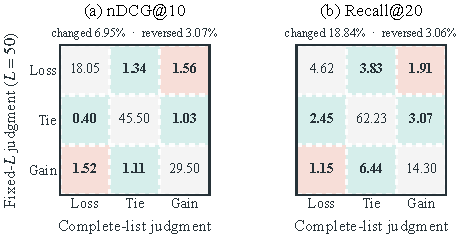
\includegraphics[width=\columnwidth]{figures/fig_fixed_top_l_diagnostics.pdf}
\caption{Transition between the DESA-versus-Original judgment at fixed
$L=50$ (rows) and under complete-list fusion (columns). Cells report the
equal-dataset percentage of query--draw pairs. Green off-diagonal cells change
among gain, tie, and loss; red cells are strict gain--loss reversals.}
\label{fig:fixed-l-diagnostics}
\end{figure}

At $L=50$, 6.95\% of nDCG judgments and 18.84\% of Recall judgments differ
from complete-list fusion. Strict gain--loss reversals account for 3.07\% and
3.06\%, respectively. Other cutoffs and ordered top-20 agreement appear in
Appendix Table~\ref{tab:cutoff-query-diagnostics}.

\subsection{Complete-List Effectiveness and Certification Depth}

Table~\ref{tab:main-results} reports the primary complete-list comparison.
DESA reaches .4747 nDCG@10 and .4695 Recall@20, gains of 3.82\% and 2.38\%
over Original. Dense and sparse certification depths fall by 36.90\% and
36.56\%, and 63.31\% of queries become shallower in both channels. All four
differences remain significant after Holm correction
($p_{\mathrm{Holm}}=.0004$).

\begin{table}[H]
\centering
\scriptsize
\setlength{\tabcolsep}{3.2pt}
\begin{tabular}{lrrrr}
\toprule
Method & nDCG@10 $\uparrow$ & Recall@20 $\uparrow$ & $L_D\downarrow$ & $L_S\downarrow$ \\
\midrule
\multicolumn{5}{l}{\textit{Original query}} \\
Original & 0.4572 & 0.4586 & 1752.4 & 1455.1 \\
\addlinespace[1pt]
\multicolumn{5}{l}{\textit{Shared expansion}} \\
Shared & 0.4671 & 0.4666 & \textbf{607.4} & \textbf{606.7} \\
\addlinespace[1pt]
\multicolumn{5}{l}{\textit{Single-channel construction}} \\
Dense only  & 0.4621 & 0.4637 & 1386.5 & 1219.9 \\
Sparse only & \underline{0.4714} & \underline{0.4678} & 884.4 & 822.0 \\
\addlinespace[1pt]
\multicolumn{5}{l}{\textit{Channel-asymmetric construction}} \\
DESA & \textbf{0.4747} & \textbf{0.4695} & \underline{728.9} & \underline{673.2} \\
\bottomrule
\end{tabular}
\caption{Equal-dataset macro results for the seven-dataset controlled
comparison. Higher is better for retrieval metrics; lower is better for replay
stopping depths. Raw depths are averaged across datasets; percentage reductions
in the text are computed within each dataset before macro-averaging.}
\label{tab:main-results}
\end{table}

Shared expansion reaches lower raw depths but also lower nDCG. Because it uses
the same references as DESA, the difference isolates how shared evidence is
integrated across channels.

\subsection{Cross-Channel Coordination}

The matched Shared comparison isolates integration while holding generated
evidence fixed. DESA improves macro nDCG by 1.61\% and Recall by 0.61\%.
The nDCG difference is significant ($+.0075$;
$p_{\mathrm{Holm}}=.0012$), whereas Recall ($+.0028$;
$p_{\mathrm{Holm}}=.2736$) and both depth differences are not. The evidence
therefore supports a quality benefit from coordinated integration, but not a
depth advantage over Shared.

The sparse channel shows why shared evidence requires coordinated integration.
Shared expansion enlarges sparse support on six datasets, by as much as
$5.72\times$. On NFCorpus, support grows from 561.5 to 3211.6 documents and
sparse depth rises by 105.81\%. DESA instead preserves virtually all Original
support while reducing sparse and dense depth by 23.15\% and 15.03\%.
Table~\ref{tab:channel-evidence} extends this contrast across datasets.

\begingroup
\definecolor{effhead}{HTML}{DCEFEA}
\definecolor{accesshead}{HTML}{E2E7F5}
\definecolor{supporthead}{HTML}{FAEDC9}
\definecolor{positive}{HTML}{E7F5F0}
\definecolor{negative}{HTML}{F3D4CE}
\definecolor{access}{HTML}{EBEEF9}
\definecolor{broaden}{HTML}{FFF2CF}
\definecolor{preserve}{HTML}{DDF2E9}
\definecolor{pattern}{HTML}{EEF0F2}
\newcommand{\effcell}[1]{\colorbox{positive}{\strut\makebox[3.25em][c]{#1}}}
\newcommand{\negcell}[1]{\colorbox{negative}{\strut\makebox[3.25em][c]{\textbf{#1}}}}
\newcommand{\accesscell}[1]{\colorbox{access}{\strut\makebox[3.25em][c]{#1}}}
\newcommand{\broadcell}[1]{\colorbox{broaden}{\strut\makebox[3.65em][c]{#1}}}
\newcommand{\keepcell}[1]{\colorbox{preserve}{\strut\makebox[3.65em][c]{#1}}}
\newcommand{\patterncell}[1]{\colorbox{pattern}{\strut\scriptsize\textbf{#1}}}
\begin{table*}[t!]
\centering
\scriptsize
\setlength{\tabcolsep}{3.0pt}
\renewcommand{\arraystretch}{1.20}
\begin{tabular}{lrrrrrrr}
\toprule
& \multicolumn{3}{c}{\colorbox{effhead}{\strut\textbf{Effectiveness: relative $\Delta$nDCG@10 (\%)}}}
& \multicolumn{2}{c}{\colorbox{accesshead}{\strut\textbf{Replay-depth reduction (\%)}}}
& \multicolumn{2}{c}{\colorbox{supporthead}{\strut\textbf{Sparse support ($\times$ Original)}}} \\
\cmidrule(lr){2-4}\cmidrule(lr){5-6}\cmidrule(lr){7-8}
\textbf{Dataset}
& \textbf{DESA vs. Orig.}
& \textbf{+Dense given Sparse}
& \textbf{+Sparse given Dense}
& $\boldsymbol{L_D}$
& $\boldsymbol{L_S}$
& \textbf{Shared}
& \textbf{DESA} \\
\midrule
SciFact
& \effcell{+2.40} & \effcell{+1.12} & \effcell{+0.91}
& \accesscell{22.2} & \accesscell{20.9}
& \broadcell{1.62$\times$} & \keepcell{1.00$\times$} \\
NFCorpus
& \effcell{+3.37} & \effcell{+2.14} & \effcell{+1.36}
& \accesscell{15.0} & \accesscell{23.2}
& \broadcell{\textbf{5.72$\times$}} & \keepcell{1.00$\times$} \\
TREC-COVID
& \effcell{+5.69} & \effcell{+0.51} & \effcell{+4.68}
& \accesscell{74.9} & \accesscell{66.7}
& \broadcell{1.53$\times$} & \keepcell{1.00$\times$} \\
FiQA
& \effcell{+3.61} & \negcell{$-$0.66} & \effcell{+3.74}
& \accesscell{49.7} & \accesscell{48.7}
& \broadcell{1.64$\times$} & \keepcell{1.00$\times$} \\
ArguAna
& \effcell{+1.27} & \effcell{+0.32} & \effcell{+0.88}
& \accesscell{15.2} & \accesscell{15.3}
& \broadcell{1.00$\times$} & \keepcell{1.00$\times$} \\
Touch\'e-2020
& \effcell{+7.52} & \effcell{+0.92} & \effcell{+5.70}
& \accesscell{45.8} & \accesscell{45.8}
& \broadcell{1.88$\times$} & \keepcell{1.00$\times$} \\
SCIDOCS
& \effcell{+0.86} & \effcell{+0.03} & \effcell{+0.13}
& \accesscell{35.4} & \accesscell{35.4}
& \broadcell{2.02$\times$} & \keepcell{1.00$\times$} \\
\midrule
\textbf{Pattern}
& \patterncell{7/7 improve}
& \patterncell{6/7 improve}
& \patterncell{7/7 improve}
& \patterncell{7/7 shallower}
& \patterncell{7/7 shallower}
& \patterncell{up to 5.72$\times$}
& \patterncell{$\approx$1.00$\times$} \\
\bottomrule
\end{tabular}
\caption{Per-dataset evidence for cross-channel coordination.
Effectiveness columns report relative nDCG@10 changes; +Dense and +Sparse
compare DESA with the corresponding one-operator construction. Depth columns
report replay stopping-depth reductions from Original, where positive values
indicate smaller certified prefixes. Sparse support is normalized by Original;
red marks the sole degradation.}
\label{tab:channel-evidence}
\end{table*}
\endgroup

The $2\times2$ comparison reveals unequal but complementary roles. Dense
expansion alone improves nDCG and Recall by 1.08\% and 1.11\%, with dense and
sparse depth reductions of 8.16\% and 7.49\%. Sparse anchoring yields gains of
3.11\% and 2.01\%, with reductions of 28.77\% and 27.74\%. Adding Sparse
anchoring to Dense only improves nDCG on all seven datasets; adding Dense
expansion to Sparse only improves six, with FiQA at $-0.66\%$. Their
combination nevertheless improves over Original and reduces both depths on
every dataset.

The matched operator controls sharpen this conclusion. Residual dense expansion
does not significantly outperform unprojected expansion, nor does score-product
anchoring significantly outperform direct sparse rewriting. Yet full DESA
improves Original on every dataset and significantly improves nDCG over Shared.
The consistent advantage therefore belongs to the coordinated construction,
not to a demonstrably superior isolated operator. Sparse-support preservation
is exact on six datasets and 99.9999\% on Touch\'e-2020, whose exported tail
omits 25 extremely low-scoring document occurrences. Angle, turnover, rank-movement,
binary-mask, reference-count, and operator-control diagnostics appear in
Appendices~\ref{sec:appendix-mechanism} and~\ref{sec:appendix-analysis}.

\subsection{Comparison with Expansion and Fusion Methods}

Table~\ref{tab:fidelity} compares DESA with matched QuDAR and reproduced
expansion methods. Under matched references, QuDAR and DESA achieve similar
complete-list effectiveness; neither paired metric difference is significant.
DESA reduces total certification depth by 74.41\% (95\% CI: 67.27--80.89;
$p_{\mathrm{Holm}}=.0002$).

\begin{table}[H]
\centering
\scriptsize
\setlength{\tabcolsep}{2.4pt}
\begin{tabular}{lrrr}
\toprule
Method & nDCG@10 $\uparrow$ & Recall@20 $\uparrow$ & Total depth $\downarrow$ \\
\midrule
\multicolumn{4}{l}{\textit{Matched references, seven datasets}} \\
QuDAR-complete & \textbf{0.4760} & \textbf{0.4712} & \underline{5478.4} \\
DESA         & \underline{0.4747} & \underline{0.4695} & \textbf{1402.1} \\
\addlinespace[1pt]
\multicolumn{4}{l}{\textit{Prior query expansion, seven datasets}} \\
Original     & 0.4572 & 0.4586 & 3207.6 \\
HyDE         & 0.4114 & 0.4374 & 16668.8 \\
MuGI         & 0.4584 & 0.4596 & 2790.1 \\
Query2doc    & \underline{0.4728} & \underline{0.4675} & \underline{1771.5} \\
DESA         & \textbf{0.4747} & \textbf{0.4695} & \textbf{1402.1} \\
\bottomrule
\end{tabular}
\caption{External comparisons over the same seven evaluation datasets. Total
depth sums the policy-specific replay depths of all rankings used by each
complete-list fusion target.}
\label{tab:fidelity}
\end{table}

Among reproduced expansion methods, DESA has the highest effectiveness and the
lowest total depth. Its closest baseline, Query2doc, is slightly lower on both
metrics and requires greater total depth. These comparisons are descriptive;
we do not claim paired significance for the lower block of
Table~\ref{tab:fidelity}.

\subsection{Robustness and Failure Boundary}

With Mistral, all four sampled datasets retain non-negative effectiveness
changes. Dense and sparse depth reductions range from 7.12\% to 47.61\% and
7.16\% to 47.62\%; 10\% of sampled ArguAna queries trigger the structured-output
fallback.

With Contriever, both effectiveness metrics improve on all four datasets.
Touch\'e-2020 nevertheless increases dense and sparse depths by 14.29\% and
4.34\%, the only setting where both worsen. TREC-COVID gains remain positive
but non-monotonic across corpus sizes. Appendix~\ref{sec:additional-results}
reports the remaining generator, encoder, reference-count, fusion, and scale
results.

\FloatBarrier

\input{sections/06-conclusion}
\input{sections/07-limitations}

\bibliography{references}

\appendix
\input{sections/a-appendix}

\end{document}
